\noindent
\rule{0.75\linewidth}{0.3pt}
\section{Threaded elements and screws}
\begin{multicols}{2}
	
	The main dimensions to consider while dealing with threaded elements are the root diameter $d_r$ (inner dimension on the screw), the major nominal diameter $d$ (measured on the external edge) and the pitch (mean) diameter $d_p$. Each thread presents an axial pitch $p$ (distance between contiguous threads), a lead $L$ (travel of a pitch for a round, integer multiple of $p$) and a helix angle $\lambda$ such that $L = \pi d_p \tan\lambda$.\\
	Usually the \textit{inclination} of the thread ($30^\circ$ in the next figure) is described by the parameter $\alpha$.
	
	\begin{center}
		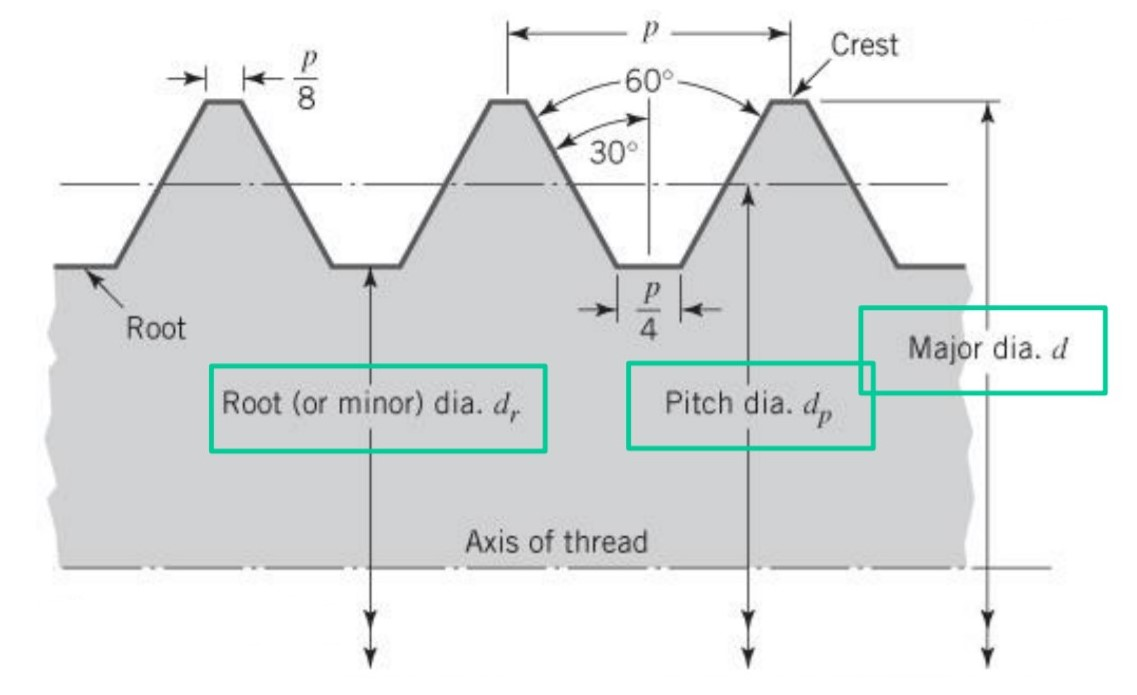
\includegraphics[width=\linewidth]{thread-profile}
	\end{center}
	
	Each standard has it's particular thread profile and values for the various parameters.

	Each screw should be described by a major (nominal) diameter (12), a length (50), a reference standard (ISO 4014) and a property class (8.8) as
	\begin{center}
		Screw \texttt{M12 x 50 ISO 4014-8.8}
	\end{center}
	In particular while defining the property class (according to ISO definitions) the first number is used to express the tensile strength in $100MPa$, while the other number (right side of the point) represent the relative percentage value of the yield strength; in the particular case of class \texttt{ISO 4014-8.8} we have a tensile strength $\sigma_r = 8\cdot 100 MPa$ and a yield of $\sigma_{ys}=0.8 \sigma_r = 640MPa$.
	
	The property class is related to the material of the threaded element, however similar concepts and codes are defined to classify both the head of the screws and the nuts.
	
\subsection{Power screws}
	Power screws use mechanical advantage of the threaded element in order to lift weights.
	\begin{center}
		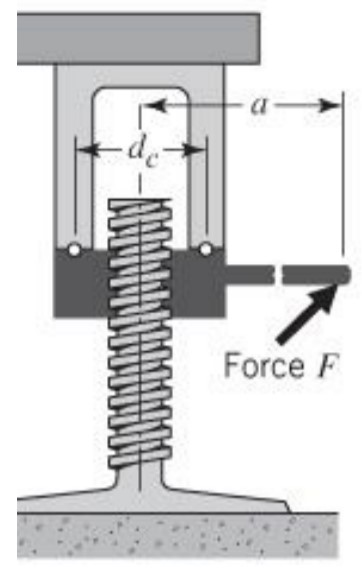
\includegraphics[width=3cm]{power-screw}
	\end{center}
	By doing a force equilibrium it's possible to compute the torque $T$ (determined by the force $F$, so $T=Fa$) that has to be transmitted in order to lift a weight $w$ is determined by the equation
	\begin{equation}
		T = \frac{w d_m}{2} \frac{f\pi d_m + \cos\alpha_n L}{-fL + \pi d_m \cos\alpha_n} + \frac{wf_cd_c}{2}
	\end{equation}
	where $f$ is the friction coefficient between the screw and the collar, $f_c$ the friction coefficient between the collar (having diameter $d_c$) and the support of the weight to be lifted, while the other parameters $\alpha_m,L,d_m$ are specific for the threaded element (as previously defined). Similarly the torque to apply in order to lower the same weight has to be equal to
	\[ T = \frac{w d_m}{2} \frac{f\pi d_m - \cos\alpha_n L}{fL + \pi d_m \cos\alpha_n} + \frac{wf_cd_c}{2} \]
	
	Power screws can be of 2 type: self locking if, with no torque applied, the system stays locked due to the friction contact between the threaded element and the lever, while in the other condition we refer the system as a overhauling screw. The condition on the friction $f$ in order to have a self locking screw is
	\[ f \geq \frac{L\cos\alpha_n}{\pi d_m} = \tan\lambda \, \cos\alpha_n \]
	The efficiency $e$ of the system that determines the ratio of the lifting power respect to the input power (considering that part of the power is dissipated by friction) is equal to
	\[ e= \frac{\cos\alpha_n - f\tan\lambda}{\cos\alpha_n + f\cot \lambda } \]
	
\subsection{Tensile bolted connection verification}
	In the case of tensile joint we can model both the screw and the members as springs (to which we have to calculate the stiffness) that are congruent, so such that the displacement $\Delta l_b$ of the bolts relates to the one of the member $\Delta l_f$ in a way such that
	\[ \textrm{interference:  } \quad i = \Delta l_b - \Delta l_f	\]
	Calculating the interference $i$ the idea is that we can compute also the preload of the bolted connection that can be used to verify the system.
	
	\begin{center}
		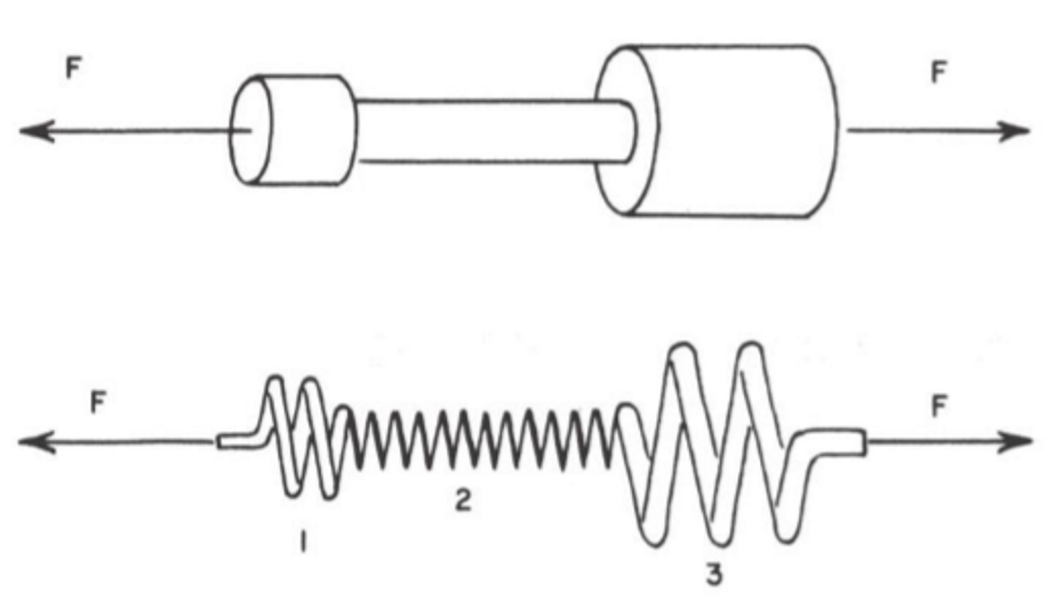
\includegraphics[width=5cm]{keq}
	\end{center} 
	
	Considering that a bolt (and as we can see later the members) can be modeled as a series of springs, the equivalent stiffness $K_b$ can be computed as
	\begin{equation}
		K_b = \left( \sum_i \frac{l_i}{E A_i} \right)^{-1}
	\end{equation}
 	While doing a bolted connection the screw elongates (in order to increase the pushing force that tighten the components) and the tensile force applied $F$ by the screws is proportional by the deformation $\Delta l_b$ of the bolt:
 	\[ F =K_b \, \Delta l_b \]
 	
 	\begin{center}
 		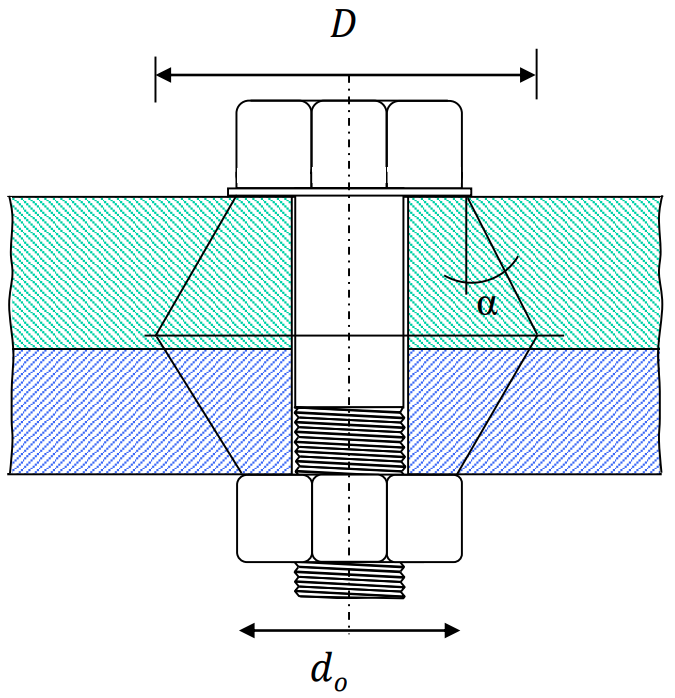
\includegraphics[width=4cm]{membstiff}
 	\end{center}  
 	
	Considering now the members determining the equivalent stiffness is harder (due to the complex behavior of the force flows), however experimental analysis determines a distribution of the tensile stress in the cone as shown in the figure above (where $\alpha$ typically measures $30^\circ$).
	\begin{center}
		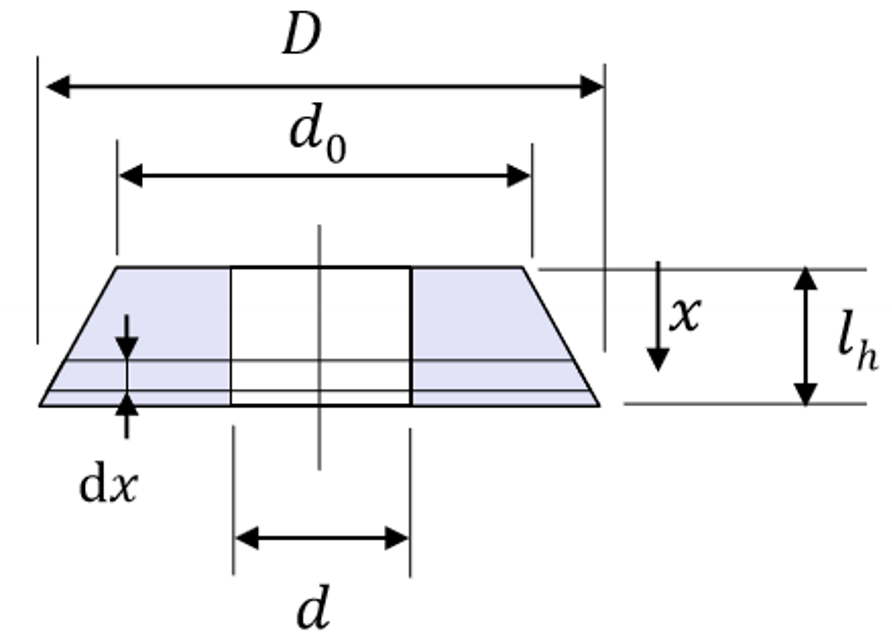
\includegraphics[width=4cm]{membstiff-det}
	\end{center}  
	By integrating the equivalent stiffness of each infinitesimal hollow cone, for every member we can compute it's equivalent stiffness as
	\begin{equation}
		K_i = \frac{\pi E d \tan \alpha}{\ln \left( \frac{D-d}{D+d} \frac{d_0+d}{d_0-d} \right)}
	\end{equation}
	Also in this case the equivalent stiffness of the member $K_f$ can be computed as $\left( \sum_i K_i \right)^{-1}$. 
	
	\begin{center}
		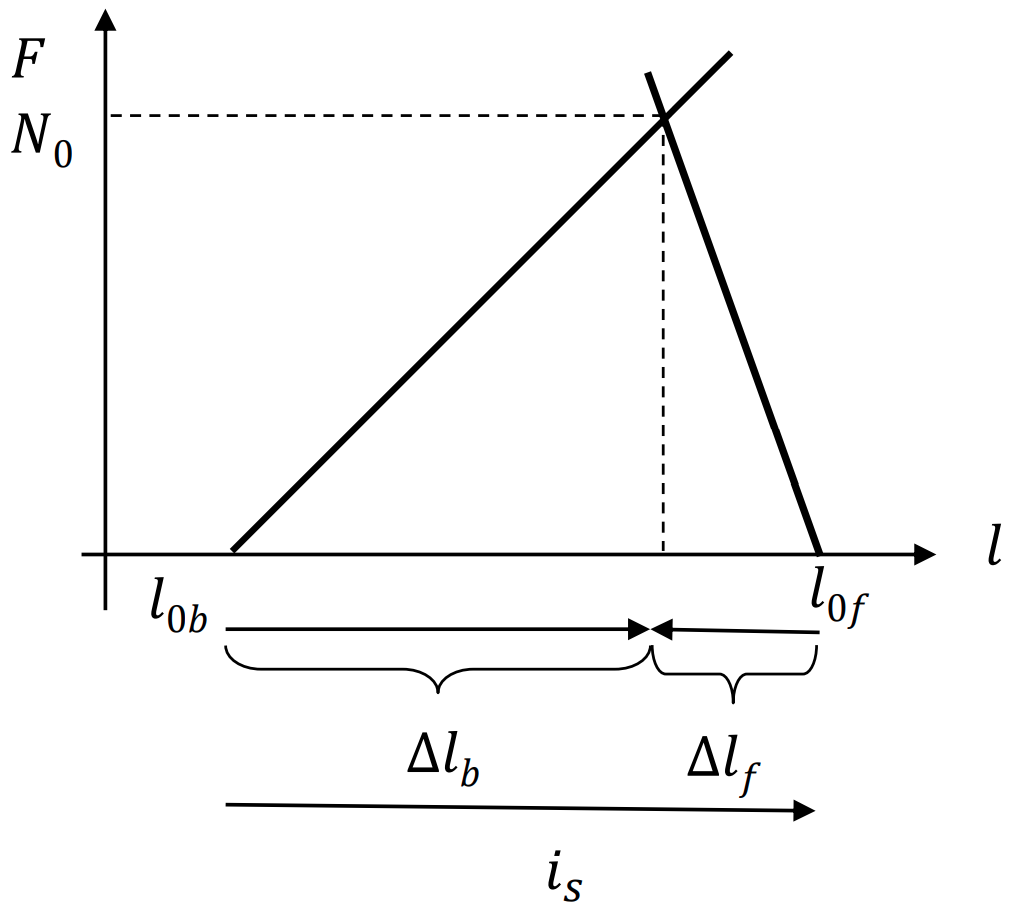
\includegraphics[width=5cm]{preload}
	\end{center}
	As in the figure above, given the resting length of the bolt $l_{0b}$ and the member $l_{0f}$ it's possible to calculate the preload force $N_0$ that's acting between the components in order to have the congruence between the two equivalent springs.
	Analytically we can define
	\[ i_s = N_0 \left( \frac{K_f + K_b}{K_fK_b} \right) \]
	
	\begin{center}
		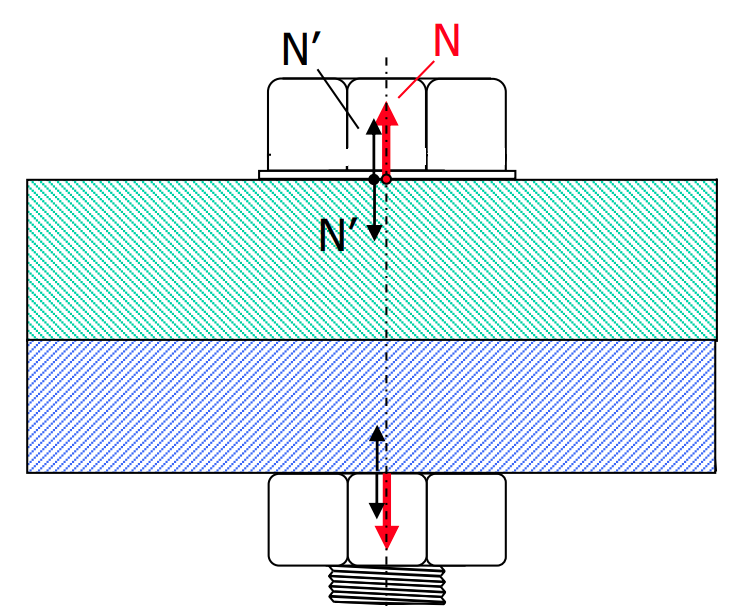
\includegraphics[width=5cm]{bolt-force}
	\end{center}

	Considering to apply now a separating load $N$ on the bolt we determine an extra elongation $\Delta l_b$ of the bolt (respect to the initial condition) while recovering the member compression. Graphically we can see how the distribution of the forces now diverges, increasing the force $N_b$ on the bolt while decreasing the preload from $N_0$ to $N'$.	
	\begin{center}
		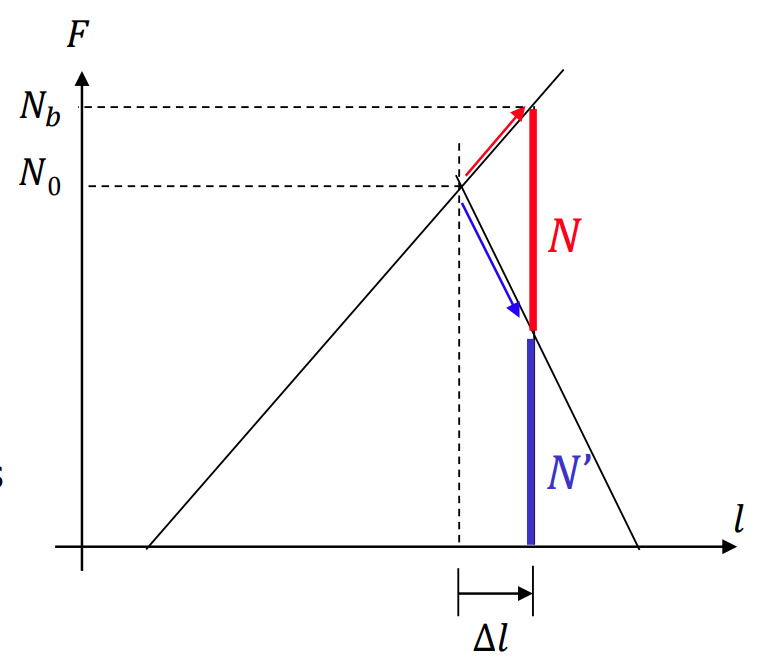
\includegraphics[width=5cm]{bolt-force-graph}
	\end{center}
	Considering the elastic model of both the members and the bolt we can compute the force $N_b$ on the screw element and the remaining tensile action $N'$ on the members as
	\[ N_b = N_0 + N \frac{K_b}{K_b+K_f} \qquad N' = N_0 + N \frac{K_f}{K_b+K_f} \]
	
	
	
	
	
	
	
	
	
	
	
	
	
	
	
	
	
	
	
	
	
	
	
	
	
	
	
	
	
	
	
	
	
	
	
	
	
\end{multicols}